% DISCUSSION CONTENT


In this work, we aimed to accelerate scientific progress in the field of single-cell omics by providing and evaluating computational tools. In section~\ref{sec:research_objectives} we proposed a concrete set of objectives this work will attempt to solve. Every chapter respectively tackles one of these research objectives, and each chapter discusses the implications of that part of our research in detail. This chapter reflects on the impact of this work on the field, going over each of the objectives and respective chapters. 


\begin{figure}[htb!]
	\centering
	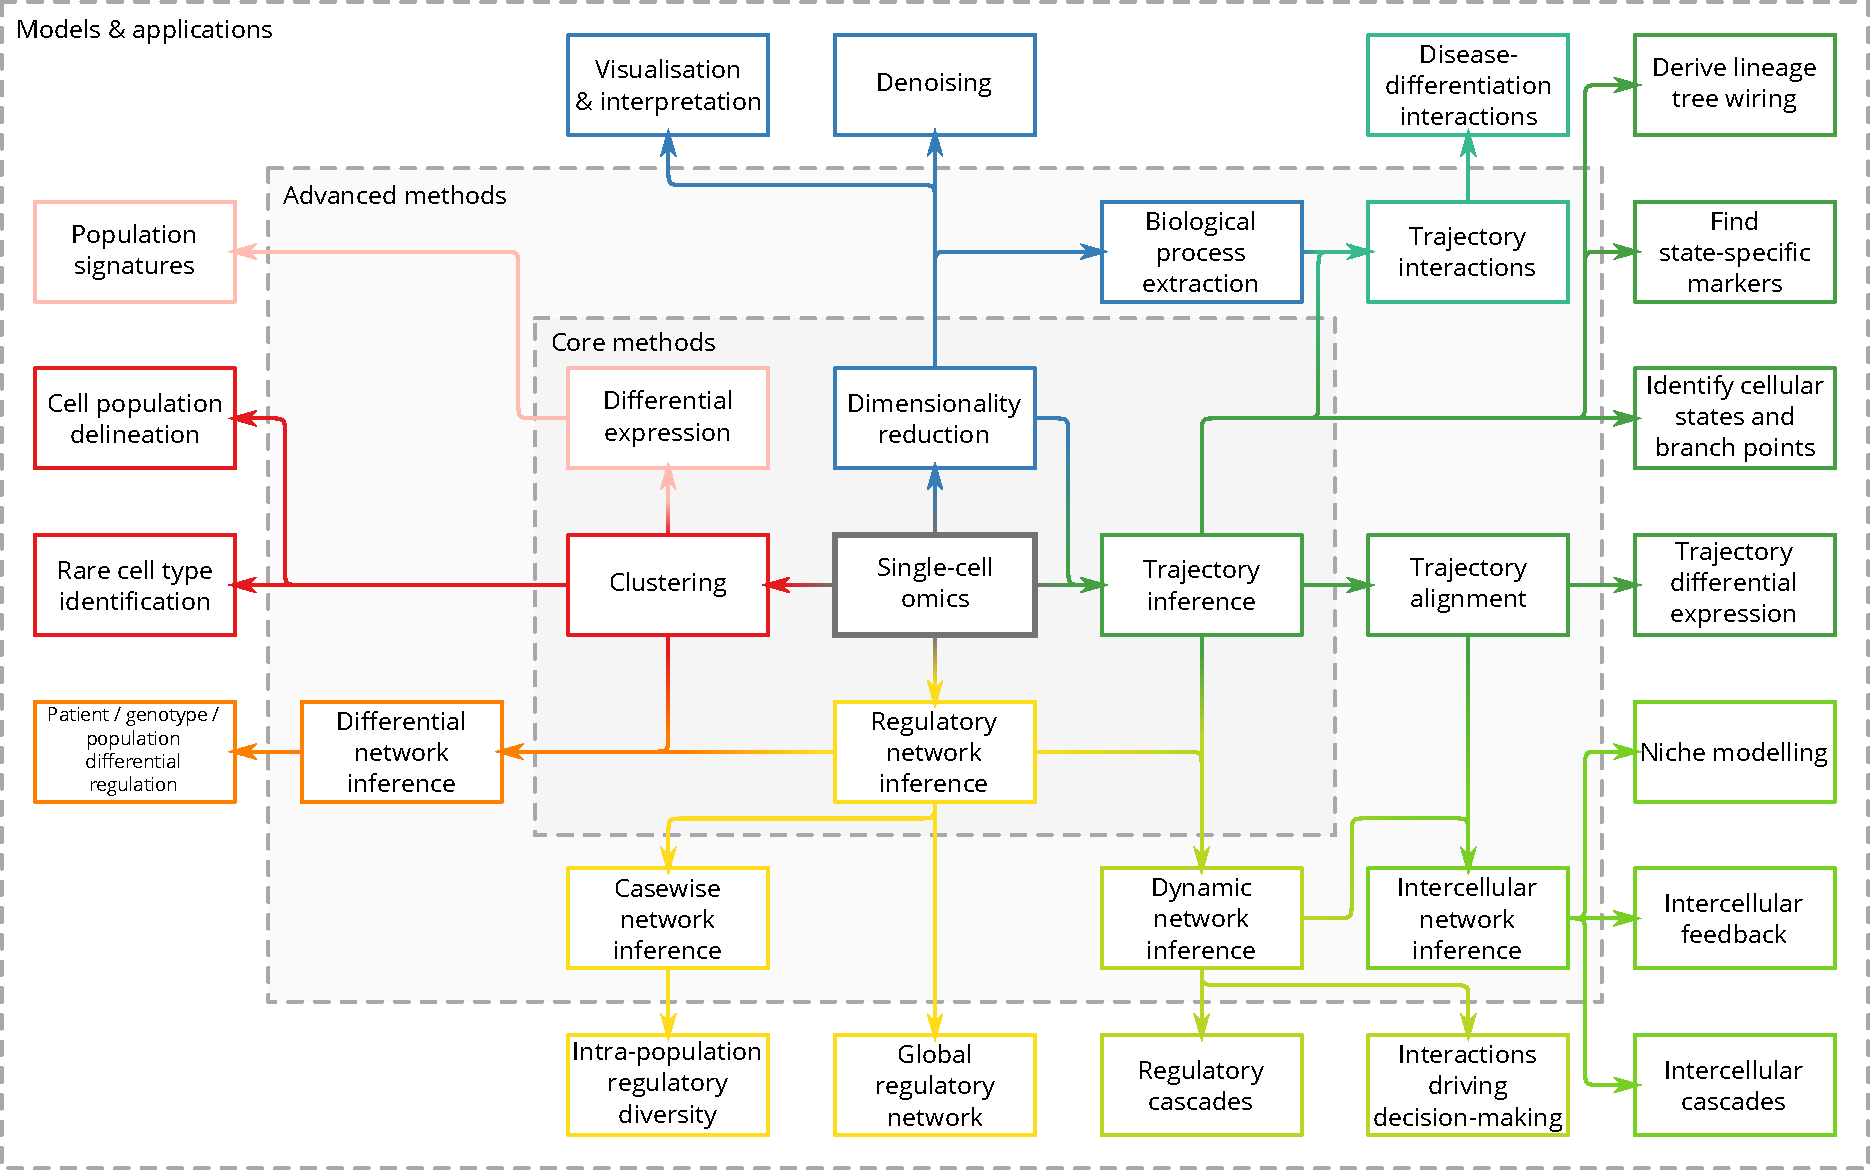
\includegraphics[width=\linewidth]{fig/singlecell_technologies_v7.pdf}
	\caption{<caption>. Adapted from work by Wouter Saelens and myself.}
	\label{fig:singlecell_technologies}
\end{figure}

\section{Trajectory inference}

\section{Network inference}

\section{Benchmarking in bioinformatics}






\section{Benchmarking with \textit{in silico} single cells}

We developed \texttt{dyngen}, a simulator of single cells to benchmark and stress-test computational tools for single-cell omics (Chapter~\ref{chap:dyngen}).
The \texttt{dyngen} software supports a selection of existing experimental protocols, and can also simulate experiments that are not possible with the current technologies, such as generating omics profiles from the same cell at multiple timepoints.
The generated data can help kick-start emerging domains with low data availability more safely by allowing software developers to test their method before numerous datasets become publicly available.

\texttt{dyngen} has already been successfully used to evaluate trajectory inference \cite{saelens_comparisonsinglecelltrajectory_2019}, trajectory alignment \cite{vandenberge_trajectorybaseddifferentialexpression_2019}, and network inference \cite{pratapa_benchmarkingalgorithmsgene_2019} methods. Furthermore, we showed that it can also be used to evaluate differential network inference methods, and trajectory alignment methods.

% Eventueel kort ook beschrijven waar je denkt dat het nog van toepassing kan zijn? The use if dyngene is not limited to.... but might also,....
% Eventueel ook: waar zie je nog verbeter/uitbreidingspunten in je methode. 
% Wat zijn de huidige limitaties. Bv. Is er een tijdgebonden limitatie. bv. Stel je wilt data van 10.000 cellen genereren maar bent een maand bezig, etc.



\section{Comparing 45 trajectory inference methods}
Using this simulator and a collection of real datasets, we performed a comparison of 45 TI methods (Chapter~\ref{chap:dynbenchmark}).
Our contributions include writing software to run 45 different error-prone TI methods with a common interface, downloading and processing hundreds of single cell datasets, and developing novel metrics for comparing ground truth and predicted trajectories.
With this benchmarking study, we had two clear goals in mind: to help guide users to TI methods that are suitable for their needs, and to provide developers of TI methods with the necessary tools to benchmark their own tool.

We accomplished the first goal by constructing a set of guidelines for end-users to help choose a TI method that is accurate, robust and fit for their application. 
Since such guidelines were hitherto lacking, they are now commonly disseminated in manuscripts \cite{lafzi_tutorialguidelinesexperimental_2018,luecken_currentbestpractices_2019}, courses \cite{kiselev_analysissinglecell_2019,martens_analysissinglecell_2019}, and slides shown during keynote caffeine refuelling sessions \cite{hemberg_coffeebreakanalysis_2019}. 

For our second goal, it seems too early to tell whether our research had any effect on self-assessments of TI method developers. We did made our pipeline, datasets, metrics, and containerised wrappers of TI methods publicly available for developers to use.
However, so far we do not observe an increase in developers performing quantitative benchmarks. We hypothesise causal reasons for this phenomenon and provide solutions in order to spur TI developers to perform more self-assessments (Chapter~\ref{chap:selfassessment}).
% "We hypothesise." Where/what do you hypothise? In your paper? Dan zou ik verwijzen naar deze sectie.
% Eventueel ook: Is there room for improvement for existing methods (deze zullen vermoedelijk onder een andere naam gepubliceerd dienen te worden)
% Dienen eerdere publicaties in vraag te worden gesteld (indien minder goede methods gebruikt werden?
% Kan dit uitgebreid worden naar andere methoden?
% Is dyngen niet ontstaan omdat je nood had aan betere datasets? Zou je in dit opzicht niet dit deeltje eerst plaatsen en verwijzen naar dyngen?
% Misschien ook vermelden dat de publicatie een aanzienlijke support verwacht van jullie team na publicatie. Dat de hoge nood gepaard gaat met een grote vraag. 
\section{A toolkit to infer, visualise and interpret single-cell trajectories}

The previous two works necessitated developing a tool for visualising trajectory data. We extended this implementation into a full toolkit, named \texttt{dyno}, for inferring and analysing trajectories (Chapter~\ref{chap:dyno}). The toolkit allows performing downstream analyses such as detecting differentially expressed genes along transitions in the trajectory, annotating the trajectory, and comparing multiple trajectories in a common dimensionality reduction. A major benefit of \texttt{dyno} is that it allows utilising any of the 50 TI methods we wrapped as part of the comparison, without having to install dependencies for every TI method separately.

The software packages consist of several subpackages, each with a separate functionality (e.g. \texttt{dynplot} visualises trajectories, \texttt{dynmethods} provides wrappers for the TI methods). Since most of the packages are currently only hosted on Github, only users familiar with Github have been able to use it. To make \texttt{dyno} available to a larger audience, we are publishing each of these packages and developing command-line interfaces for the most important functionalities.

% Are we talking about R-packages?


\section{Fast, accurate, and robust single-cell pseudotime}

We developed a TI method, called \texttt{SCORPIUS}, specialised in inferring linear trajectories (Chapter~\ref{chap:scorpius}). Since our comparison of TI methods already lists 30 TI methods that can infer trajectories that are more complex than a linear ordering of cells, why would we need a linear TI method?

Being able to study how cells progress over time is in terms of analysis as fundamental as being able to cluster cells or to identify differentially expressed genes between two groups. We showed that for analysing datasets containing linear trajectories, \texttt{SCORPIUS} outperforms all other TI methods tested as part of our TI benchmark. 

Despite \texttt{SCORPIUS} published on bioRxiv in 2016, discussion and usage of the pre-print has largely been limited to comparing the results of a different (linear) TI methods to those of \texttt{SCORPIUS}. Since the pre-print, many improvements have been made to improve the accuracy and robustness of predicted trajectories, to allow scaling up to datasets containing 100'000s of cells, and to providing a more user-friendly interface. Since the beginning of 2019 -- before the publication of our benchmark of TI methods -- several studies have now reported using \texttt{SCORPIUS} as a tool for deriving primary results \cite{damond_maphumantype_2019, cheng_multifactorialheterogeneityvirusspecific_2019, tibbitt_singlecellrnasequencing_2019, hove_singlecellatlasmouse_2019, wouters_singlecellgeneregulatory_2019, reimegard_combinedmrnaprotein_2019}.


\section{Inferring single cell regulatory networks}

We proposed a novel algorithm for inferring case-wise gene regulatory interactions (Chapter~\ref{chap:bred}). While we demonstrated the methodology by inferring 14'963 sample-specific GRNs from the TCGA project, further interpretation of these results needs to be perform to validate the usefulness of the method.

Additional avenues for exploration could involve applying trajectory inference on the case-wise regulome data, and quantitatively evaluating the performance of the algorithm using the \texttt{dyngen} simulations.

\section{Optimising regulatory networks}
This project was a spin-off of Netter \cite{ruyssinck_netterrerankinggene_2016}, a tool for reranking GRN predictions using structural network properties. 
Predicted GRNs often are topologically dissimilar to real networks, and as such, Netter quantifies the topological properties of a network and makes incremental changes in order to arrive at a network with a 'better' topological profile.

The topological 'profile' of a network was defined as the frequencies of particular topological patterns called 'graphlets'. Keeping track of the frequencies of graphlets during an iterative process proved difficult at first. 
\texttt{incgraph} provides a solution to this problem (Chapter~\ref{chap:incgraph}) by  assuming that the incremental changes between two different networks are relatively small (less than 100 edge additions/removals). Under this assumption, it is possible to calculate the differences in topological patterns significantly faster in comparison to recomputing the graphlet frequencies from scratch at every iteration.

While \texttt{incgraph} solved a very specific and interesting problem, and was eventually published as a peer-reviewed article, it has not succeeded in making a direct impact on scientific research as of yet. Perhaps, at some point, a researcher will come across \texttt{incgraph} and find that it exactly solves his or her problem.

% Of je dient voor te stellen bij welke dataset het goed van toepassing is en het te promotor onder de Vlaamse research gemeenschap?


\section{A life without Git, Travis CI, or tidyverse}
A significant portion of this work involved developing large software libraries, in a collaborative setting, over a time span of about four years. Since the results of our comparison of 45 TI methods required three years to develop, we were happily forced to develop a system where experiments could be rerun and results could be updated on-the-fly.

We summarised our experiences in the form of a set of guidelines for benchmarking computational tools (Chapter~\ref{chap:guidelines}). However, these guidelines do not touch upon many aspects of good software development practices that we learned to use in order to bring this thesis to a good end. In particular, I would like to highlight several  fundamental (open-source) projects without the likes of which our research would have been simply impossible to perform, namely Git, Travis CI, and the tidyverse.

\textbf{Git} \cite{torvalds_gitfastversion_2005} is a code-revision system that allows multiple users to collaborate on developing code and keep track of what changes were made by whom. 
Since Wouter Saelens and I were often working closely together on a specific part of our software, Git saved us a lot of time by merging together changes developed in parallel. Only in few cases did we need to intervene manually to merge our changes.
Additionally, Github.com allowed us not only to collaborate with each-other, but also correspond and collaborate with other software developers from many different research groups, using Github Issues to discuss problems with other researchers, and Github Pull Requests to contribute code to open-source projects. 

Together, we published over 20'000 code contributions (commits) across 50+ software packages \cite{cannoodt_developmentdynverse_2019}. Since many of these packages depend on one another, it is inevitable that changes made to one package would break another package. We wrote many, many unit tests (and still too few), and we let these tests automatically be executed on \textbf{Travis CI} \cite{traviscigmbh_traviscitest_2011}. This way, when we pushed breaking changes to Github, Travis CI would notify that our commit has resulted in one or more unit tests failing. While sometimes it is a hassle to set up, Travis CI has prevented us countless times from generating faulty results due to a faulty underlying function.

Software bugs can be introduced even by incredibly small, seemingly insignificant changes. The R programming language seems particularly susceptible towards getting trapped by its many pitfalls. However, there are many benefits of using R in bioinformatics research context, such as its extensive community of statisticians develop packages for the R ecosystem. The \textbf{tidyverse} packages \cite{wickham_welcometidyverse_2019}, developed by the RStudio team and many online contributors, completely transformed my experiences with R from tedious struggles to efficient everyday functional programming.

Honourable mentions go to Linux, Fedora, \LaTeX, TeXstudio, (R)Markdown, Bash, Sed, Regular expressions, Rocket Chat, for making bioinformatics software development even more fun and enjoyable.

% ideas:
%  Yet I wonder how the current academic system
%can support such concepts. Academics often hold different positions in
%different research groups around the world, who should be the maintainer in
%these cases? The original PhD students that developed the work? The original
%research group?

%The eight chapter is a manuscript in preparation about the assessment of TI methods. The main discussion topic is the lack of a quantitative measure for the scoring of new TI methods. This leads to the publication and development of new methods that do not show a clear performance improvement compared to other methods. The main topic touches
%upon some sore points that are inherent in bioinformatics. The main thought I have with
%this chapter is that defining clear goals in an emerging technology is difficult and therefore is sometimes ignored by fellow bioinformaticians. This because the lack of standardized performance metrics, missing public datasets that are well described and an \textit{ad hoc} problem definition. I follow the idea of defining a clear cut approach to benchmarking (as described in chapter nine) and I like the proposition that is started in this manuscript for a discussion on good TI metrics.} Would approaches like e.g. DREAM challenges be a means of tackling these issues to your opinion?

% zie peter dawyndt, chapter 5
\clearpage
\section{References}
\printbibliography[heading=none]
